%%%%%%%%%%%%%%%%%%%%%%%%%%%%%%%%%%%%%%%%%
% Beamer Presentation
% LaTeX Template
% Version 1.0 (10/11/12)
%
% This template has been downloaded from:
% http://www.LaTeXTemplates.com
%
% License:
% CC BY-NC-SA 3.0 (http://creativecommons.org/licenses/by-nc-sa/3.0/)
%
%%%%%%%%%%%%%%%%%%%%%%%%%%%%%%%%%%%%%%%%%

%----------------------------------------------------------------------------------------
%	PACKAGES AND THEMES
%----------------------------------------------------------------------------------------

\documentclass{beamer}

\mode<presentation> {

% The Beamer class comes with a number of default slide themes
% which change the colors and layouts of slides. Below this is a list
% of all the themes, uncomment each in turn to see what they look like.

%\usetheme{default}
%\usetheme{AnnArbor}
%\usetheme{Antibes}
%\usetheme{Bergen}
%\usetheme{Berkeley}
%\usetheme{Berlin}
%\usetheme{Boadilla}
%\usetheme{CambridgeUS}
%\usetheme{Copenhagen}
%\usetheme{Darmstadt}
%\usetheme{Dresden}
%\usetheme{Frankfurt}
%\usetheme{Goettingen}
%\usetheme{Hannover}
%\usetheme{Ilmenau}
%\usetheme{JuanLesPins}
%\usetheme{Luebeck}
%\usetheme{Madrid}
%\usetheme{Malmoe}
%\usetheme{Marburg}
%\usetheme{Montpellier}
%\usetheme{PaloAlto}
%\usetheme{Pittsburgh}
%\usetheme{Rochester}
\usetheme{Singapore}
%\usetheme{Szeged}
%\usetheme{Warsaw}

% As well as themes, the Beamer class has a number of color themes
% for any slide theme. Uncomment each of these in turn to see how it
% changes the colors of your current slide theme.

%\usecolortheme{albatross}
%\usecolortheme{beaver}
%\usecolortheme{beetle}
%\usecolortheme{crane}
%\usecolortheme{dolphin}
%\usecolortheme{dove}
%\usecolortheme{fly}
%\usecolortheme{lily}
%\usecolortheme{orchid}
%\usecolortheme{rose}
%\usecolortheme{seagull}
%\usecolortheme{seahorse}
%\usecolortheme{whale}
%\usecolortheme{wolverine}

%\setbeamertemplate{footline} % To remove the footer line in all slides uncomment this line
%\setbeamertemplate{footline}[page number] % To replace the footer line in all slides with a simple slide count uncomment this line

%\setbeamertemplate{navigation symbols}{} % To remove the navigation symbols from the bottom of all slides uncomment this line
}
\usepackage{subcaption}
\usepackage[normalem]{ulem}
\usepackage{mathtools}
\usepackage{amsmath}
\usepackage{adjustbox}
\usepackage{graphicx} % Allows including images
\usepackage{booktabs} % Allows the use of \toprule, \midrule and \bottomrule in tables
\usepackage{tikz}
\usetikzlibrary{arrows,automata}

\graphicspath{{../plots/}}

\newcommand{\com}[1]{}

\newcommand*\pooritem{%
	\item[\color{red}\scalebox{0.9}{\textbullet}]}
\newcommand*\gooditem{%
	\item[\color{blue}\scalebox{0.9}{\textbullet}]}

%\newcommand{\gooditem}[1]{\setbeamercolor{item}{fg=blue}\item #1} 
%\newcommand{\pooritem}[1]{\setbeamercolor{item}{fg=red}\item #1} 
%\setbeamercolor{itemize/enumerate body}{parent=structure}
\DeclarePairedDelimiter\abs{\lvert}{\rvert}%
\DeclarePairedDelimiter\norm{\lVert}{\rVert}%
%----------------------------------------------------------------------------------------
%	TITLE PAGE
%----------------------------------------------------------------------------------------

\title[Too many corrections]{Too many corrections: Semantic reference-less evaluation for Grammatical Error Correction} % The short title appears at the bottom of every slide, the full title is only on the title page

\author{Leshem Choshen \& Omri Abend} 
\institute[Hebrew University Jerusalem Israel] % Your institution as it will appear on the bottom of every slide, may be shorthand to save space
{
Hebrew University Jerusalem Israel\\ % Your institution for the title page
}

\date{September 25 2017} % Date, can be changed to a custom date

\begin{document}

\begin{frame}
\titlepage % Print the title page as the first slide
\end{frame}

%\begin{frame}
%\frametitle{Overview} % Table of contents slide, comment this block out to remove it
%\tableofcontents % Throughout your presentation, if you choose to use \section{} and \subsection{} commands, these will automatically be printed on this slide as an overview of your presentation
%\end{frame}
\AtBeginSection[]
{
	\begin{frame}<beamer>
		\frametitle{Plan}
		\tableofcontents[currentsection]
	\end{frame}
}
%----------------------------------------------------------------------------------------
%	PRESENTATION SLIDES
%----------------------------------------------------------------------------------------
\begin{frame}
	\frametitle{Overview} % Table of contents slide, comment this block out to remove it
	\tableofcontents % Throughout your presentation, if you choose to use \section{} and \subsection{} commands, these will automatically be printed on this slide as an overview of your presentation
\end{frame}

%------------------------------------------------
\section{The task}
\begin{frame}
		\frametitle{\only<2>{\textcolor{green}{T}}\only<1>{t}he task}
	\begin{itemize}
		
		\item Input: a text which is perhaps \only<1>{ungramatical} \only<2>{\sout{ungramatical}} \only<2>{{\color{green}ungrammatical}}
		\item Output: a grammatical text \only<1>{saying}\only<2>{\sout{saying}} \only<2>{\textcolor{green}{conveying}} the same meaning/content.
	\end{itemize}
	\vfill
	\small
	Example:
	However , there are \only<1>{both sides of stories}\only<2>{\sout{both sides of stories}} \only<2>{$\rightarrow$\\
		However , there are \textcolor{green}{two sides to every story.}}
	
\end{frame}

%------------------------------------------------
\section{General performance on the task - Over conservatism}
\begin{frame}
	\frametitle{Current systems hardly change}
It is a virtue to avoid bad corrections, but correcting is still the goal...
	 \begin{columns}[T]
	 	\begin{column}{.5\textwidth}
	 		\begin{block}{}
	 			
	 			\begin{itemize}
	 				\item Less words changed
	 				\item Less word order changes
	 				\item Less sentences split into two
	 				\item Less sentences merged into one
	 				\item and so on...
	 			\end{itemize}
	 		\end{block}
	 	\end{column}
	 	\begin{column}{.5\textwidth}
	 		\begin{block}{}
	 			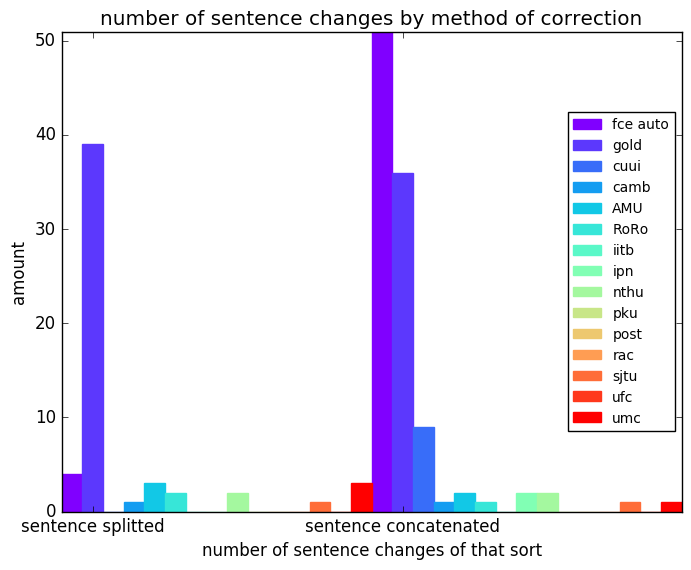
\includegraphics[width = \textwidth]{aligned}
	 		\end{block}
	 	\end{column}
	 \end{columns}
\end{frame}
\com{
\begin{frame}
	\frametitle{Current systems hardly change \emph{sentence boundaries}}
	\begin{figure}
		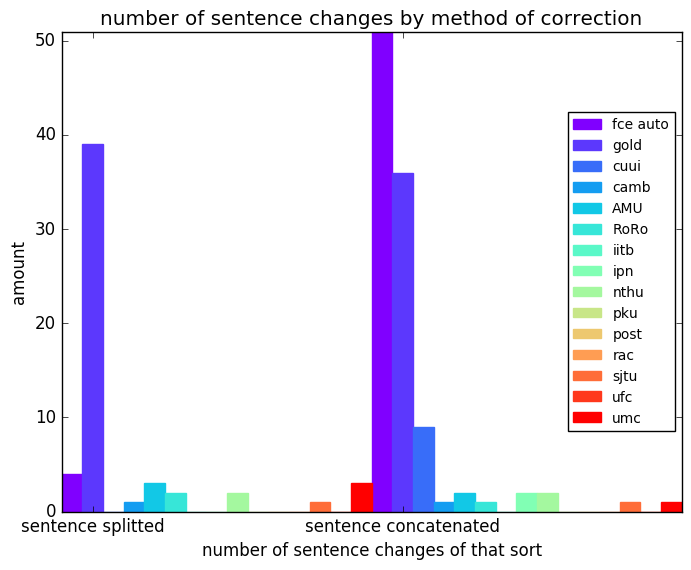
\includegraphics[width = 0.8\textwidth]{aligned}
	\end{figure}
\end{frame}
\begin{frame}
	\frametitle{Current systems hardly change \emph{words}}
	\begin{figure}
		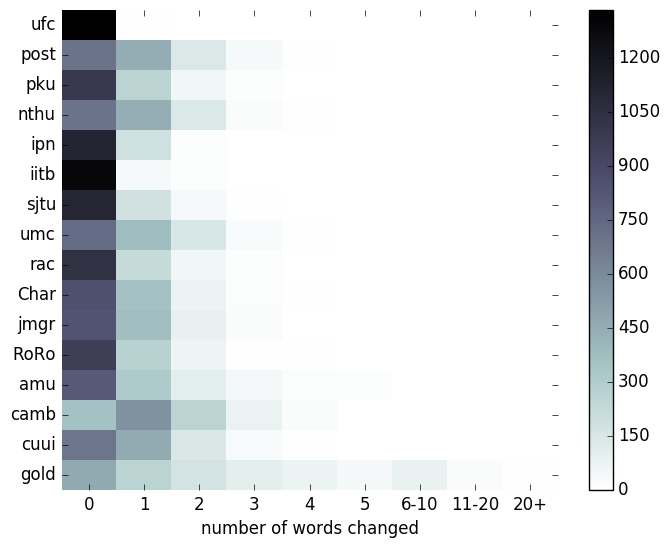
\includegraphics[width = 0.8\textwidth]{words_differences_heat}
	\end{figure}
\end{frame}
\begin{frame}
	\frametitle{Current systems hardly change \emph{word order}}
	\begin{figure}
		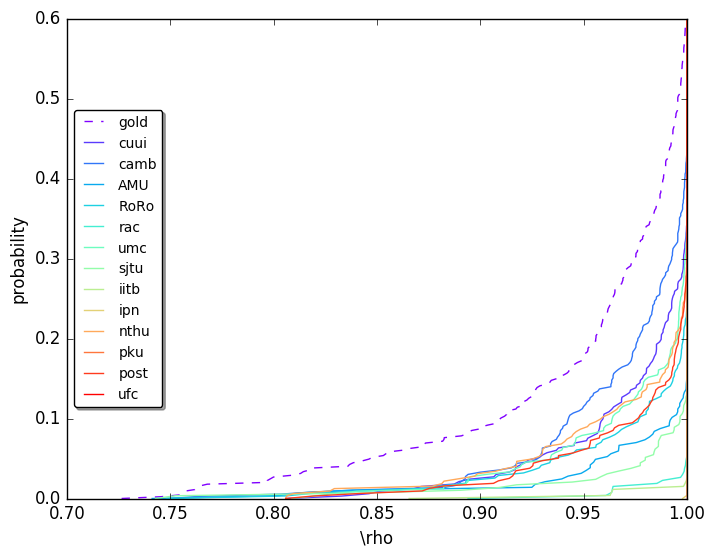
\includegraphics[width = 0.8\textwidth]{spearman_ecdf}
	\end{figure}
\end{frame}
\begin{frame}
	\frametitle{Conservatism? Over-conservatism?}
	It is a virtue to avoid bad corrections, \\but the goal is still to correct...
\end{frame}
}
%------------------------------------------------
\section{Evaluation measures - Reference based measures (RBM)s}
\subsection{Background and motivation}
\begin{frame}[label=RBM]
	\frametitle{What exists}
	Evaluation measures all share in common:
	\begin{itemize}
	\item Compare a system correction to a set of references.
	\item Emphasize precision over recall.
	\end{itemize}
	
	Corpora:
	\begin{itemize}
	\item Train and validation - 1 reference per source sentence, never more.
	\end{itemize}
\end{frame}

\begin{frame}
	\frametitle{Corrections as distribution}
	\begin{itemize}
		\item Each sentence $x$ has a set of valid corrections $correct_x$
		\item $\mathcal{D}_x$ a distribution of human corrections
		\item In a Corpus - $Y\sim \mathcal{D}_x^M$ a sample of $M$ references 
		\item $P_{coverage}$ - $P_{y\sim \mathcal{D}_x}(y \in Y)$
	\end{itemize}
\end{frame}
\begin{frame}[label=Dists]
	\frametitle{Distributions as we get from crowdsourcing}
	\begin{itemize}[<+->]
		\item Hypothesis: Probably more than 2 references, and they are not uniform but approximately so.
		\item Result: On average 1351.24 corrections per sentence with 8-15 words with a heavy tail like behaviour.
	\end{itemize}	
\end{frame}
\begin{frame}
	\frametitle{Analytical worries}
	Oracle chooses whether to produce a correction or not.\\
	Mistake detected: incentivized to correct it only if 
	$$p_{correct} \cdot p_{coverage} > 1-p_{detect} $$
	Or, given $\alpha$ punishment for wrong corrections
	$$p_{correct} \cdot p_{coverage} - \left(1-p_{correct}\cdot p_{coverage}\right) \alpha > 1-p_{detect}$$
	
	\begin{figure}

		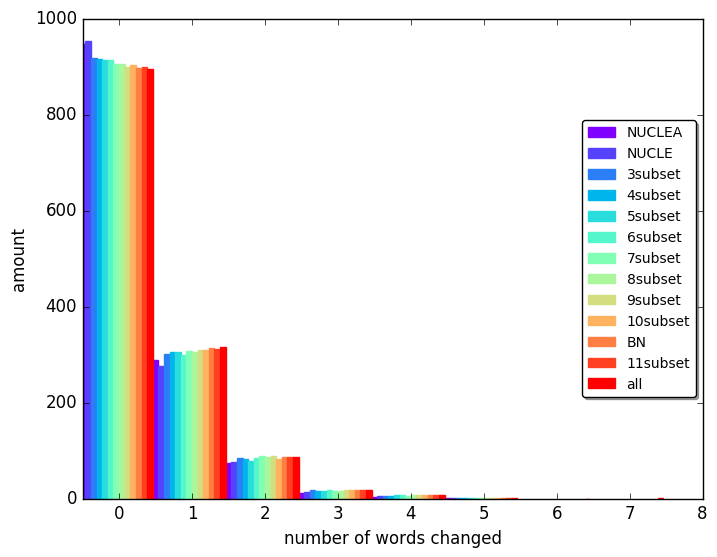
\includegraphics[width=4cm]{words_differences_hist_reranking}
				\caption{Also, empirical worries, for decoration}
	\end{figure}
\end{frame}
\com{
\begin{frame}
	\frametitle{Empirical confirmation}
	\begin{figure}
		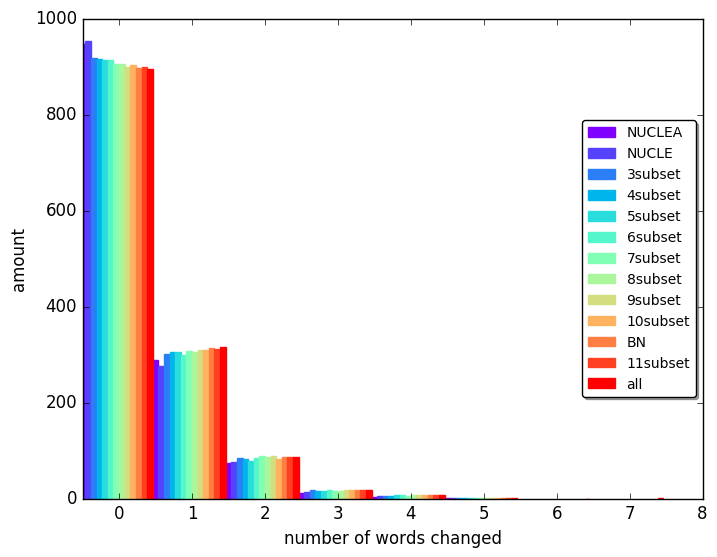
\includegraphics[width=8cm]{words_differences_hist_reranking}
	\end{figure}
\end{frame}
}

\subsection{Corrections as distribution}
\com{
\begin{frame}
	\frametitle{Estimating $\mathcal{D}$}
	To estimate $\mathcal{D}$ we use UnseenEst.
	It estimates the histogram minimizing earthmover distance.
\end{frame}
\begin{frame}[label=Dists]
	\frametitle{Findings}
	\begin{table}[h!]
		\begin{tabular}{c|c|c|c|c|}
			%\cline{2-5} 
			& \multicolumn{4}{c|}{Frequency Threshold ($\gamma$)}\\ 
			%\cline{2-5} 
			& \multicolumn{1}{c}{0} & \multicolumn{1}{c}{0.001} & \multicolumn{1}{c}{0.01} & \multicolumn{1}{c|}{0.1}
			\\
			\hline
			Variants & 1351.24 & 74.34 & 8.72 & 1.35
			\\
			Mass & 1 & 0.75 & 0.58 & 0.37\\
			\hline
		\end{tabular}
	\end{table}\hyperlink{alldists}{\beamerbutton{dists}}
\end{frame}
}
\com{
\begin{frame}
	\frametitle{Yet more findings}
	\framesubtitle{Rare corrections still count}
	\begin{figure}
		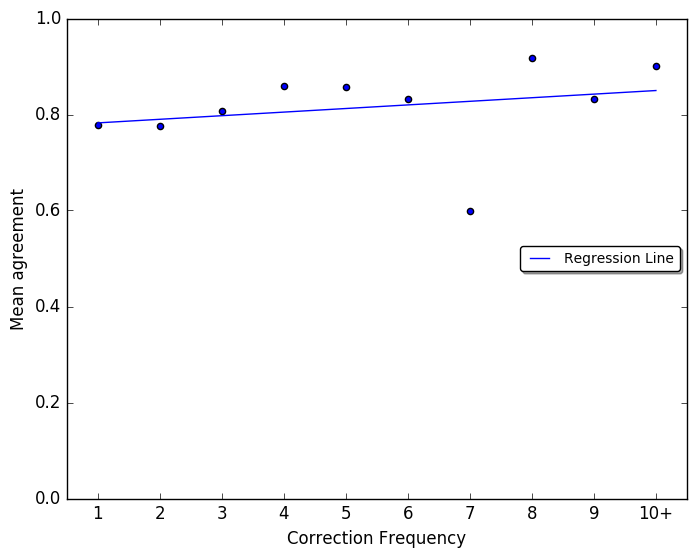
\includegraphics[width=8cm]{IAA_confirmation_frequency}
	\end{figure}
\end{frame}
}
\subsection{RBMs under estimation as a function of $M$}
\begin{frame}
	\frametitle{Accuracy - analysis}
	Given a perfect corrector, how well will it do?
	$\frac{1}{N}\sum_{i=1}^N P_{Y \sim \mathcal{D}_i^M, y \sim \mathcal{D}_i}\left(y \in Y\right)$
	\begin{figure}
		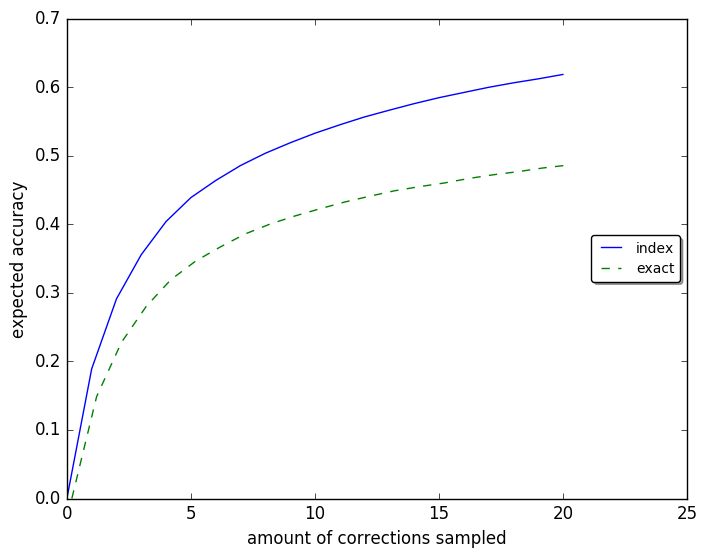
\includegraphics[width=8cm]{noSig_repeat_1000_accuracy}
	\end{figure}
\end{frame}
\begin{frame}
	\frametitle{$F_{0.5}$-score - empirical}
		\begin{figure}
			\includegraphics[width=8cm]{$F_{0.5}$_Ms_significance}
		\end{figure}
\end{frame}
\begin{frame}
	\frametitle{human vs. machine - test on 2 references}

	\begin{figure}
		\includegraphics[width=8cm]{$F_{0.5}$_significance}
	\end{figure}
\end{frame}
\section{Reference-less semantic measure}
\begin{frame}
	\frametitle{Reference-less evaluation}
	Input: Corrected sentences and Source sentences \sout{and references in the form of sentences}.
	
	Output: A score, but which?!
\end{frame}
\com{
\begin{frame}
	\frametitle{Reference-less evaluation}
	Compare the source and the correction
	\begin{itemize}
		\gooditem Suggestion: compare grammar annotations
		\pooritem Grammar is ill defined with ungrammatical text
		\pooritem Some define grammar on ungrammatical text as reference some as source
	\end{itemize}
\end{frame}
}
\begin{frame}
	\frametitle{Reference-less evaluation}
	Combine two measures
	\begin{enumerate}
		\item faithfulness -- semantic similarity of the correction and the source. \footnote{\tiny Leshem Choshen and Omri Abend. "Conservatism and Over-conservatism in Grammatical Error Correction" - under revision}
		\item grammaticality -- error detection over the source \footnote{\tiny Napoles Courtney, Keisuke Sakaguchi, and Joel Tetreault. "There's No Comparison: Reference-less Evaluation Metrics in Grammatical Error Correction." arXiv preprint arXiv:1610.02124 (2016).}
	\end{enumerate}
\end{frame}

\begin{frame}
	\frametitle{UCCA}
	\begin{itemize}
		\item Semantic annotation scheme that builds on
		typological and cognitive linguistic theories
		\item Provides a coarse-grained, cross-linguistically
		applicable representation
		\item Structures are DAGS, words are leaves
	\end{itemize}
\end{frame}
\com{
\begin{frame}[label=distances-details]
	\frametitle{Measures}
	\begin{itemize}
		\item IAA - percentage of Nodes with same label and leaves
		\item UCCASim - percentage of Nodes with same label and most matched leaves
		\item Top down - size of the biggest cut
		\item Token - Consider only main entities
		\item (Labeled) Tree edit - tree distance when ordered by tokens alignment 
	\end{itemize}
	\hyperlink{distances}{\beamerbutton{distances table}}
\end{frame}
}
\begin{frame}[label=UCCA]
	\frametitle{Ungrammatical hypotheses}
	\begin{itemize}
		\item Ungrammatical text can be annotated using UCCA
		\item Corrections change grammar, not semantics
	\end{itemize}
\end{frame}

\begin{frame}
	\frametitle{UCCASim(ilarity) between source and reference}
	\begin{table}
		\begin{tabular}{c|c|}
			& {\sc UCCASim}
		\\
		\hline
		Different annotators & 0.84 
		\\
		Same annotator & 0.92
		\\
		TUPA parser & 0.7
		\\
		\hline
		\hline
		Ungrammatical IAA & 0.83 
		\\
		Baseline IAA \footnotemark[1]\footnotetext[1]{UCCA IAA improved since the original paper} & 0.79
		\\
		TUPA reported precision & 0.69 
		\\
		\hline
		\end{tabular}
	\end{table}
\end{frame}
\com{
\begin{frame}
	\frametitle{Works also automatically (TUPA parser)}
	\begin{table}
		\begin{tabular}{c|c|c|c|}
			\cline{2-4} 
			& \multicolumn{3}{c|}{\sc UCCASim} \\
			\cline{2-4}
			& s$\rightarrow$r & r$\rightarrow$s & Avg\
			\\
			\hline
			TUPA & 0.7 & 0.7 & 0.7
			\\
			\hline
			\hline
			Different & 0.85 & 0.83 & 0.84
			\\
			\hline
		\end{tabular}
	\end{table}
\end{frame}
}
\begin{frame}
	\Huge{\centerline{Thank you}}
\end{frame}
\end{document} 